\chapter{Methodology}
\label{Chapter3}
\lhead{Chapter 3. \emph{Methodology}}

\section{Pipeline Overview}
Let $X=\{x_i\}_{i=1}^{N}$ and $Y=\{y_j\}_{j=1}^{M}$ be source and target point clouds. Dense correspondence assigns each source point a target index through a map $T:\{1,\ldots,N\}\rightarrow\{1,\ldots,M\}$. Figure~\ref{fig:current-pipeline} presents the modules that compute this map and the supervision used to learn their representations.

Preprocessing converts each shape into a point cloud with heat-based descriptors and coordinate channels. The orientation module estimates relative yaw and aligns the target. A shared ASMAE learns geometric point features through masked cross-shape reconstruction. The visual branch extracts DINOv2 descriptors from projected views and transfers their information to the learned point representation. HADM fuses the geometric and visual features, identifies consistent anchors and refines the source through non-rigid deformation before dense assignment.

\begin{figure}[H]
\centering
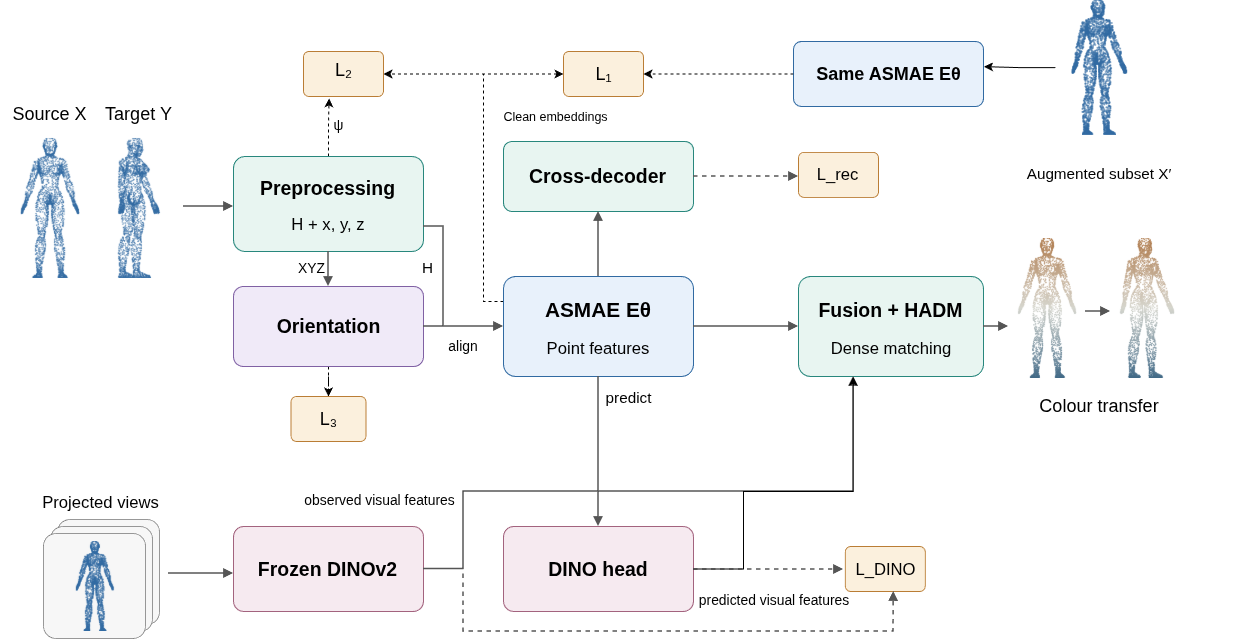
\includegraphics[width=\textwidth]{current/pipeline-overview.png}
\caption[Correspondence pipeline and training objectives.]{Correspondence pipeline and training objectives. Dashed connections identify supervision; solid connections show the flow of features and geometry. Here $L_1=L_{\mathrm{self}}$ is the self-identity objective; $L_2$ groups $L_{\mathrm{cycle}}$, $L_B$, $L_{\mathrm{orient}}$ and $L_{\mathrm{sep}}$; and $L_3$ groups the orientation objectives $L_{\mathrm{bin}}$, $L_{\mathrm{res}}$, $L_{\mathrm{subset}}$ and $L_{\mathrm{domain}}$. The colour-transfer pair illustrates how a dense point map transfers a source attribute to its corresponding target points.}
\label{fig:current-pipeline}
\end{figure}

\section{Point-Cloud Preprocessing}
\subsection{Surface points and neighbourhood graph}
The preprocessing module extracts vertex positions from the input shape and represents them as an unordered point cloud. Coordinates are centred and normalized to provide a consistent scale. A nearest-neighbour graph connects spatially nearby points, and its undirected adjacency matrix $A$ defines the graph Laplacian
\begin{equation}
 L=D-A,
\end{equation}
where $D$ is the diagonal degree matrix. Eigenpairs $(\lambda_\ell,\phi_\ell)$ describe variation over the graph and provide the spectral basis for the geometric descriptors. Figure~\ref{fig:preprocessing} shows the conversion from surface geometry to the input feature matrix.

\begin{figure}[H]
\centering
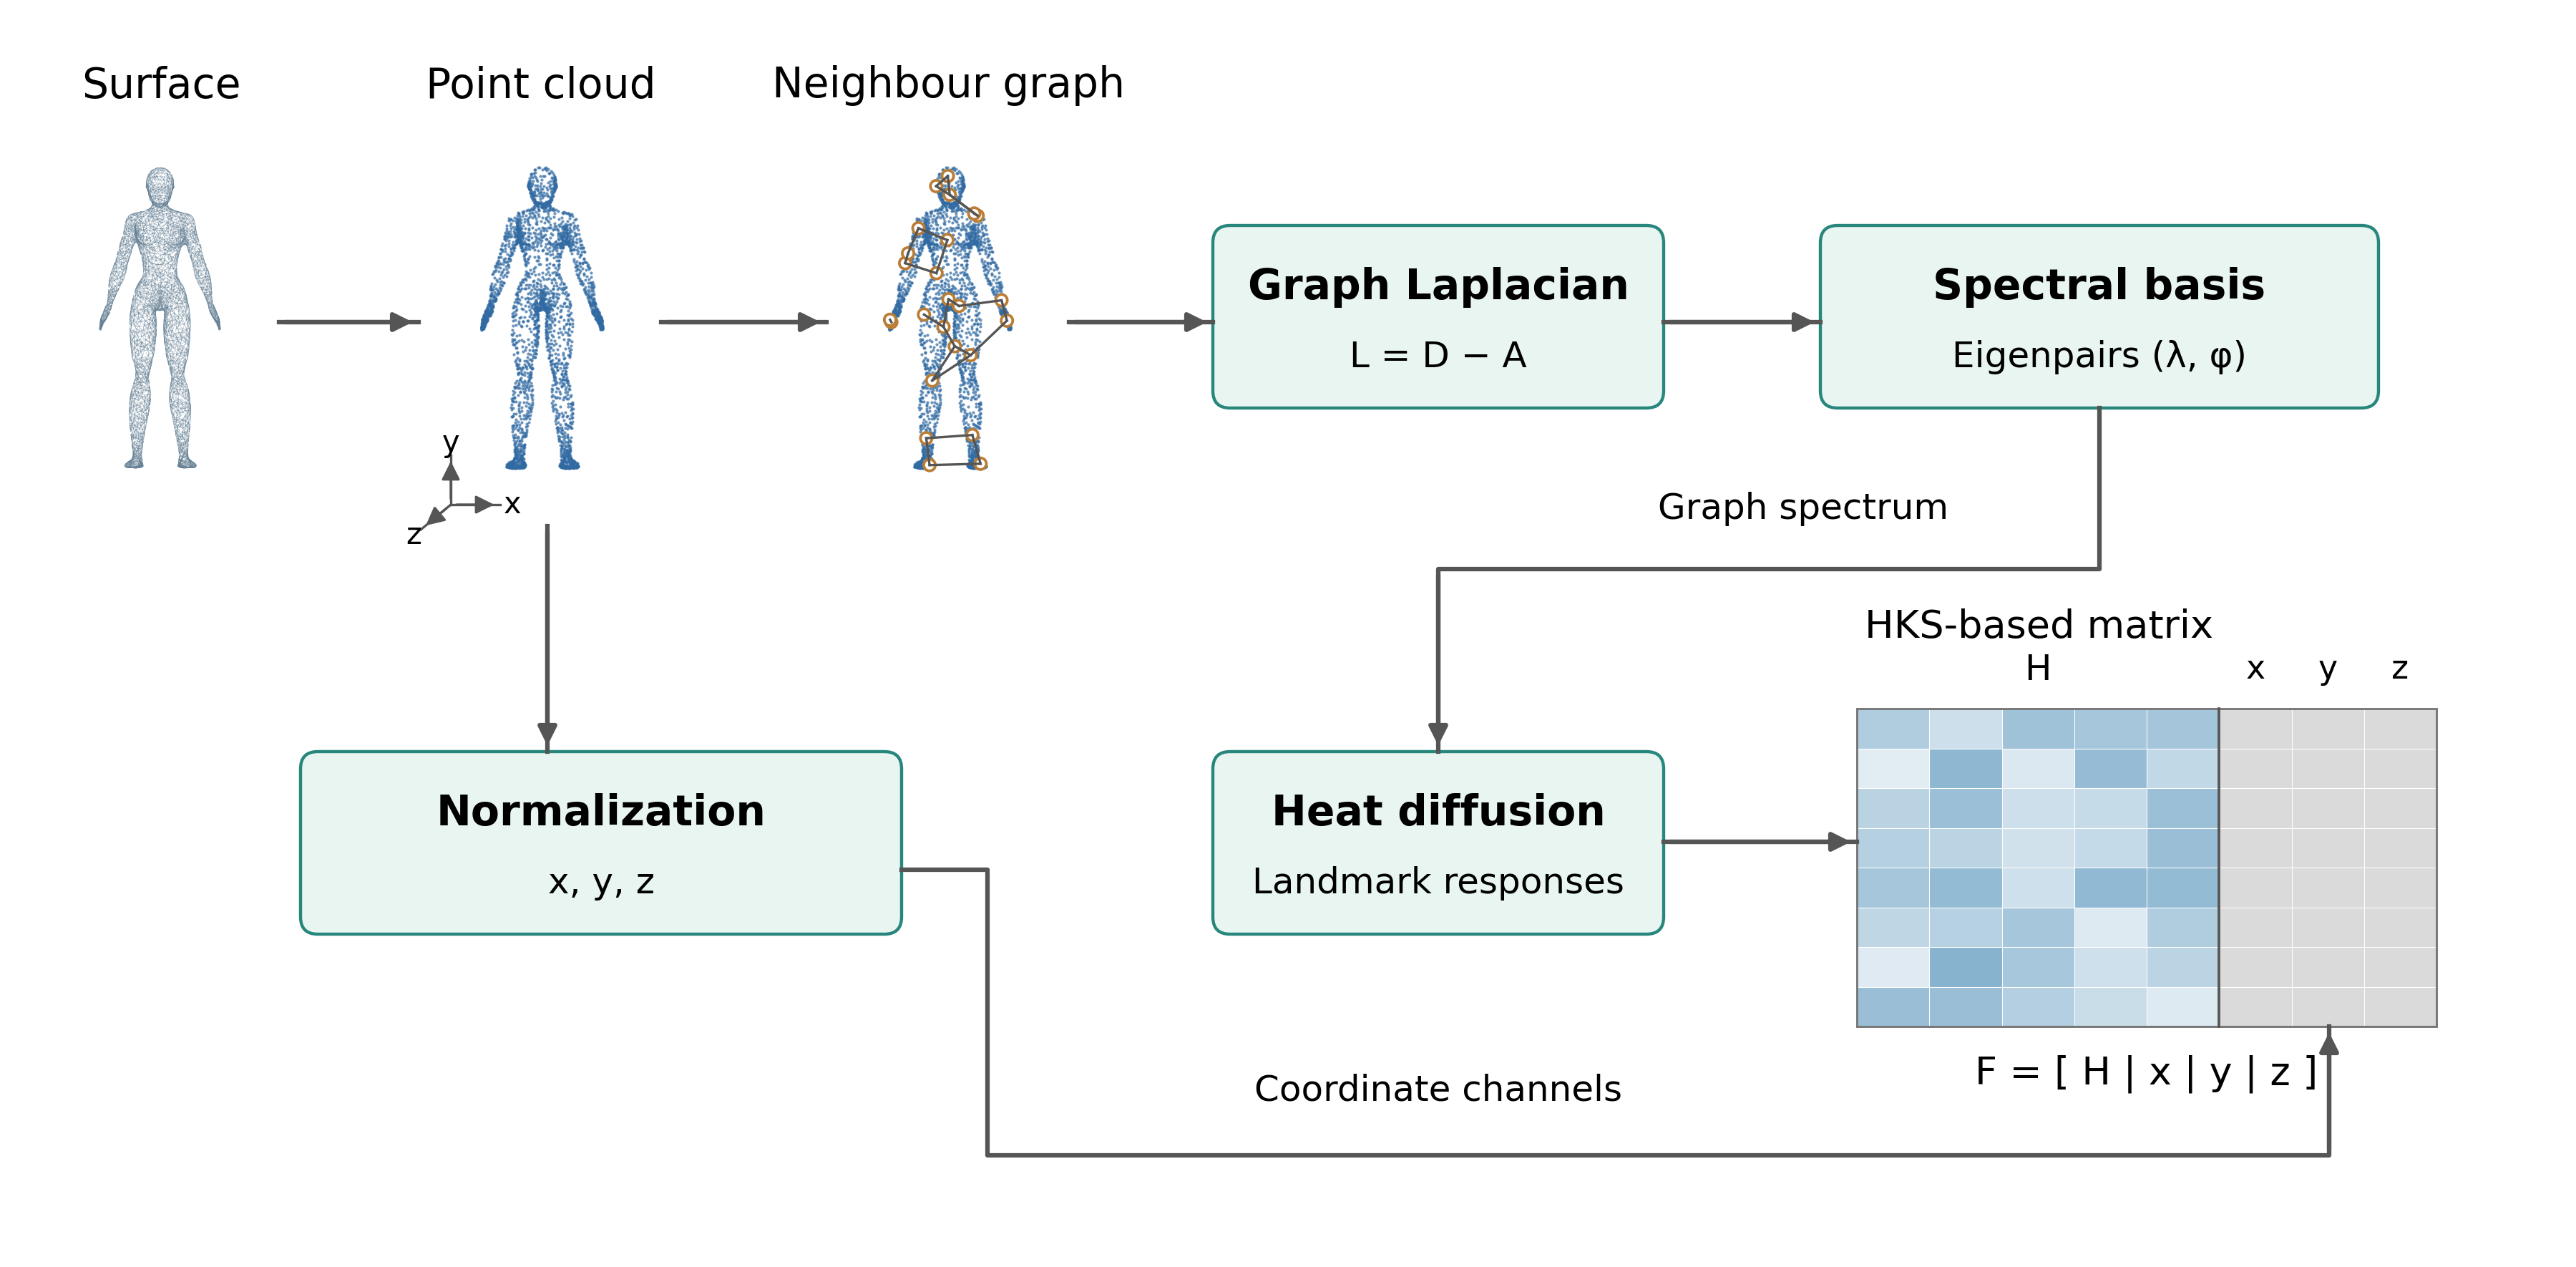
\includegraphics[width=\textwidth]{current/preprocessing.png}
\caption[Point-cloud and heat-descriptor preprocessing.]{Point-cloud and heat-descriptor preprocessing. Sampled surface positions form the point cloud and neighbourhood graph. The graph spectrum produces the heat-based descriptor matrix $H$, which is concatenated with normalized $x$, $y$ and $z$ coordinates. Matrix shading illustrates the organization of descriptor channels.}
\label{fig:preprocessing}
\end{figure}

\subsection{Heat descriptors and coordinate channels}
Heat diffusion describes how information spreads between locations on the graph. For sampled landmarks $s_1,\ldots,s_q$, the descriptor at point $x_i$ is
\begin{equation}
 H_{ij}=K_t(x_i,s_j)=\sum_\ell e^{-t\lambda_\ell}
 \phi_\ell(x_i)\phi_\ell(s_j).
\label{eq:landmark-heat}
\end{equation}
This HKS-based representation uses landmark heat responses \citep{10.5555/1735603.1735621}. Each row corresponds to a point, and each column records diffusion from a landmark. Channel normalization and logarithmic scaling balance the descriptor magnitudes.

The encoder input concatenates the heat matrix with explicit coordinates:
\begin{equation}
 F_X=[H_X\mid x\mid y\mid z].
\end{equation}
The coordinate channels supply position information alongside the spectral descriptor. They are expressed in the same frame as the point positions passed to the encoder. After relative alignment, the target coordinate channels are updated accordingly.

\subsection{Intrinsic geometric embedding}
A biharmonic embedding supplies distances for geometric regularization and anchor consistency \citep{Lipman_2010_Biharmonic}:
\begin{equation}
 \psi(x)=\left[\frac{\phi_1(x)}{|\lambda_1|},\ldots,
 \frac{\phi_r(x)}{|\lambda_r|}\right],\qquad
 d_B(x,x')=\|\psi(x)-\psi(x')\|_2.
\end{equation}
Nonzero spectral modes define the embedding, which is normalized by a reference distance scale. The resulting representation describes the relative separation of points through the graph geometry.

\section{Relative Orientation Module}
\subsection{Pairwise encoding and feature interaction}
The orientation estimation module (OEM) takes independently sampled subsets of the source and target. Shared point encoding extracts local features, and cross-shape feature interaction relates regions of one shape to the other. Global pooling produces a pair representation for predicting relative yaw about the vertical axis. The architecture follows the orientation-learning principle of SE-ORNet \citep{Deng_2023_CVPR}.

\begin{figure}[H]
\centering
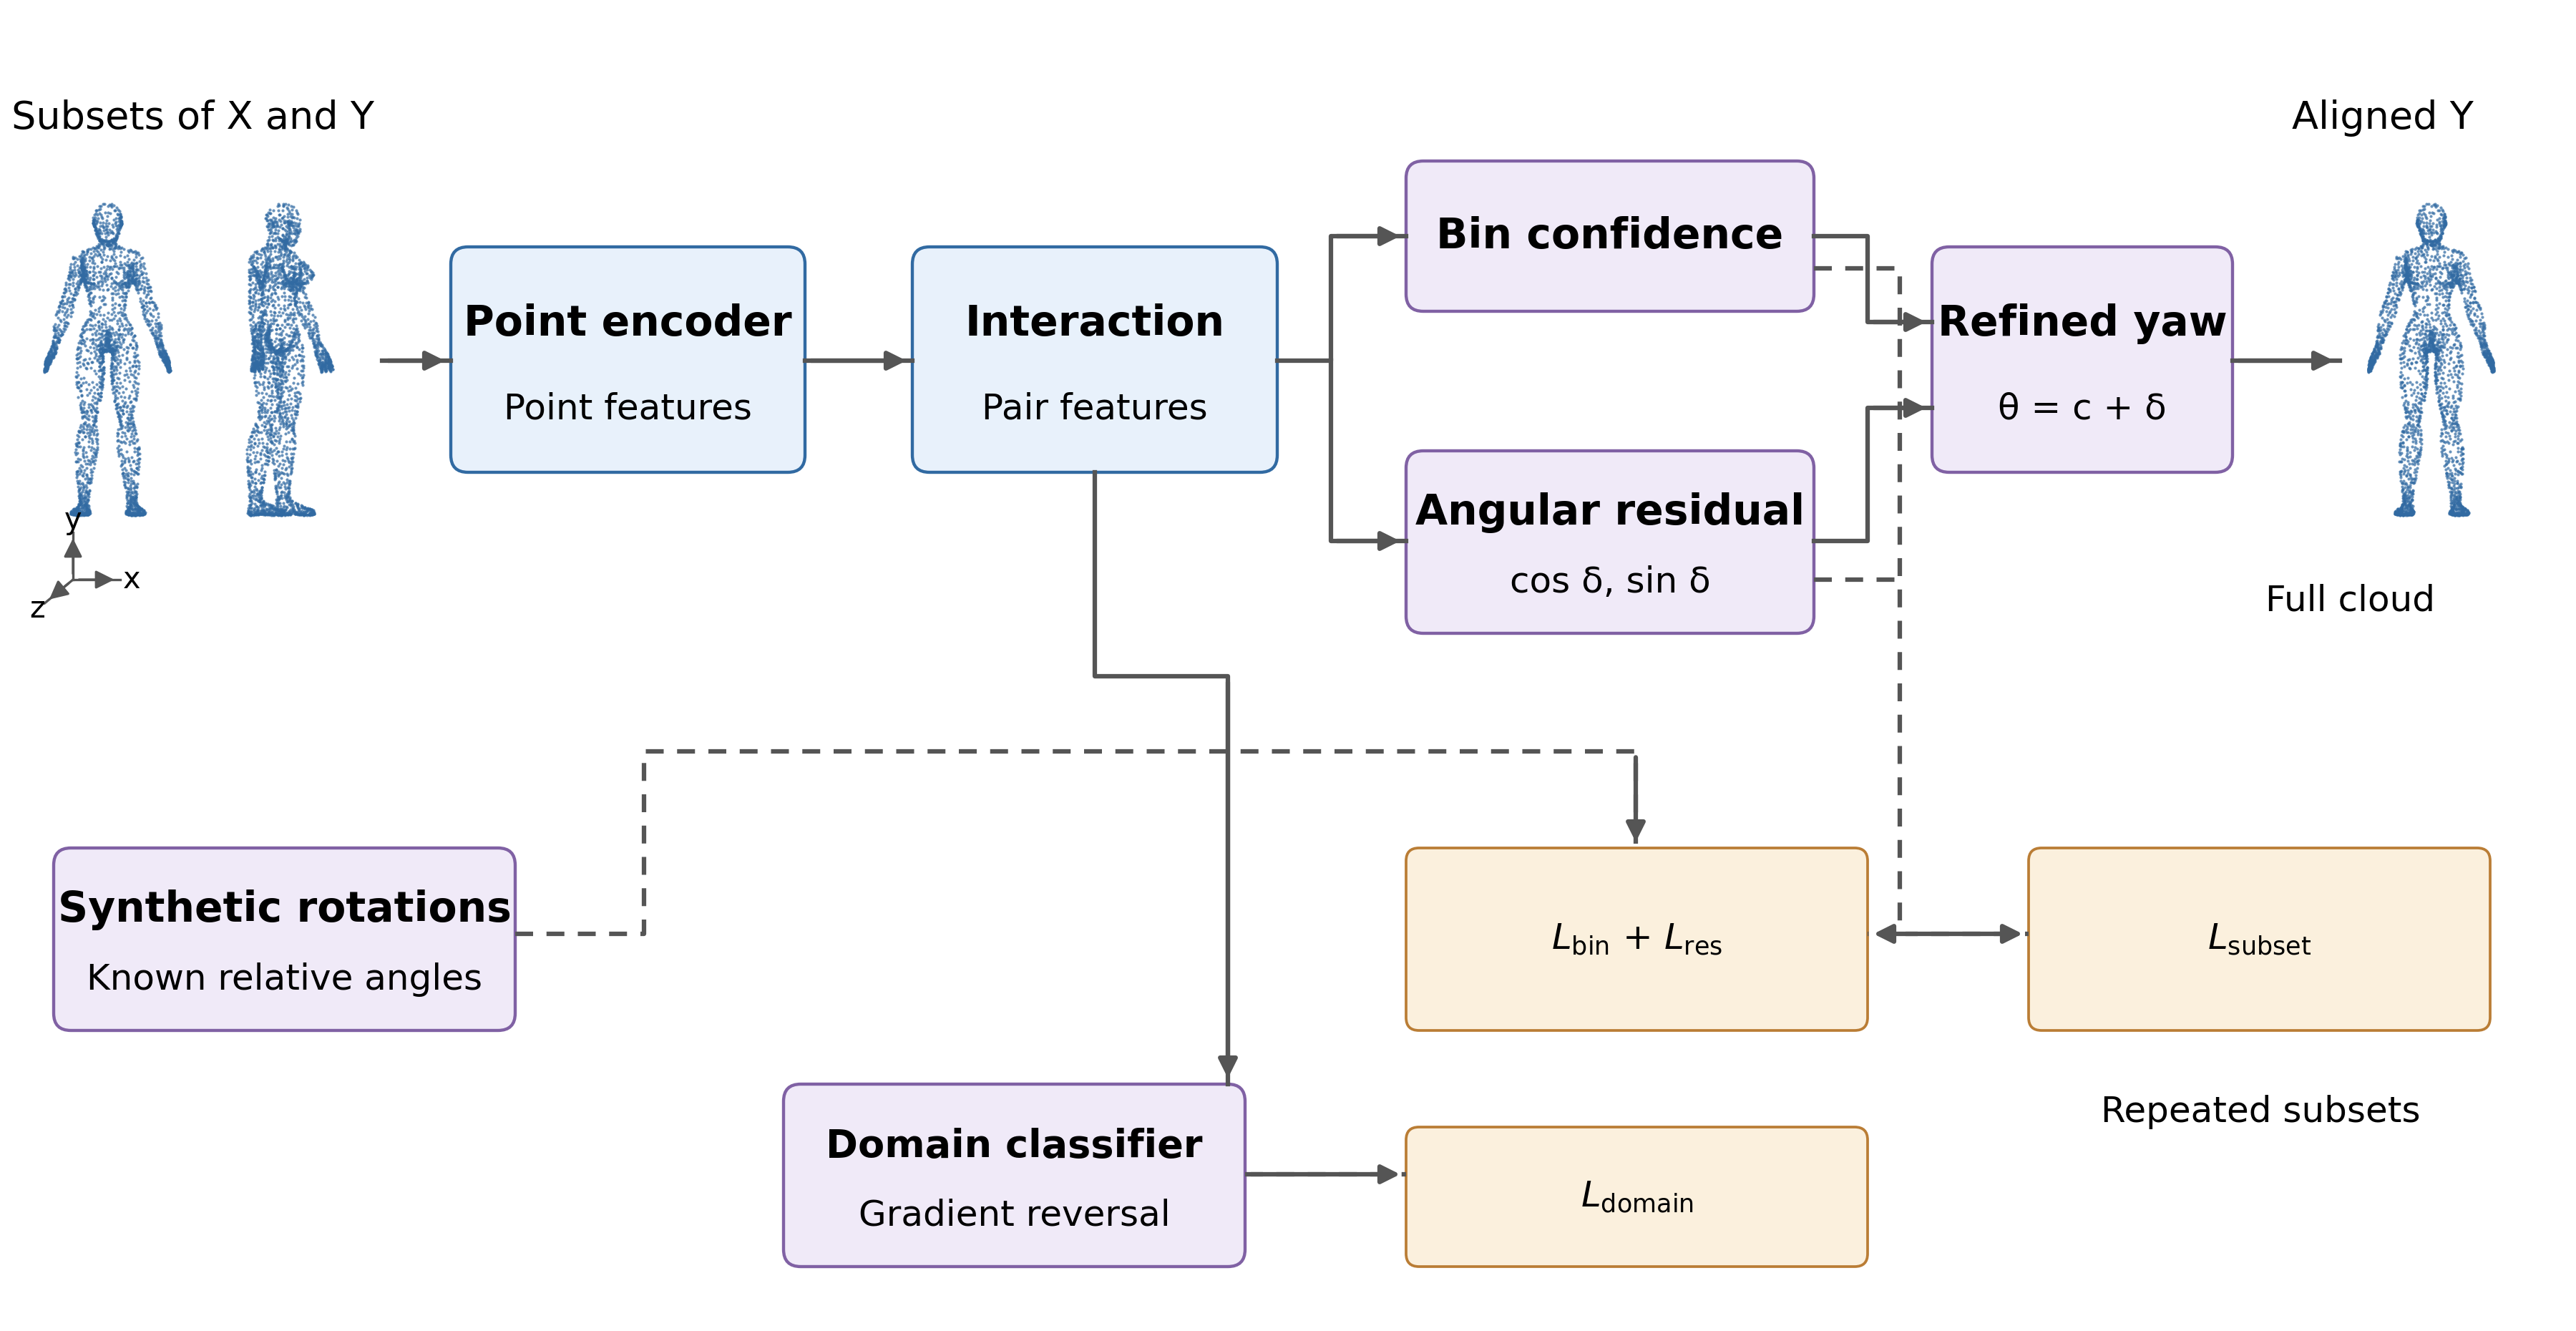
\includegraphics[width=\textwidth]{current/orientation-module.png}
\caption[Relative orientation estimation.]{Relative orientation estimation. Pairwise point features predict angular-bin confidence and a continuous residual. Synthetic rotations supervise angle prediction, repeated point subsets supply consistency supervision, and a domain discriminator connects synthetic and cross-shape pairs. The predicted yaw aligns the full target point cloud.}
\label{fig:orientation}
\end{figure}

\subsection{Continuous angular prediction}
Overlapping angular bins provide coarse orientation hypotheses. For each bin with centre $c_k$, the network predicts confidence $p_k$ and a normalized residual vector $r_k$. Following the MultiBin principle \citep{Mousavian_2017_MultiBin}, the residual represents the displacement from the bin centre through cosine and sine. The predicted angle is
\begin{equation}
 k^*=\arg\max_k p_k,\qquad
 \hat\theta=c_{k^*}+\operatorname{atan2}(r_{k^*,2},r_{k^*,1}).
\end{equation}
The residual supports continuous alignment between bin centres. Overlap allows a boundary angle to be represented by neighbouring bins. The inverse predicted rotation aligns all target points with the source frame.

\subsection{Orientation supervision}
Synthetically rotating a shape produces a paired observation with a known relative angle. Forward and inverse directions supervise the bin probabilities and residuals. Independently sampled observations of the same pair provide a consistency objective on both outputs. A gradient-reversal discriminator distinguishes synthetic same-shape pairs from cross-shape pairs \citep{JMLR:v17:15-239}; focal loss weights this domain classification \citep{Lin_2017_ICCV}.

The orientation objective combines angular classification, residual prediction, subset consistency and domain adaptation. Alignment is detached when supplying coordinates to the correspondence branch, so OEM is trained by its dedicated supervision while ASMAE is trained by representation objectives.

\section{ASMAE Representation Learning}
\subsection{Shared geometric encoder}
ASMAE maps the input heat descriptors and XYZ coordinates to point embeddings. A feature projection and a positional encoding initialize the point tokens. Local attention aggregates neighbouring tokens, with relative geometric direction supplying an attention bias. Both shapes pass through the same encoder parameters, placing their descriptors in a common feature space.

\begin{figure}[H]
\centering
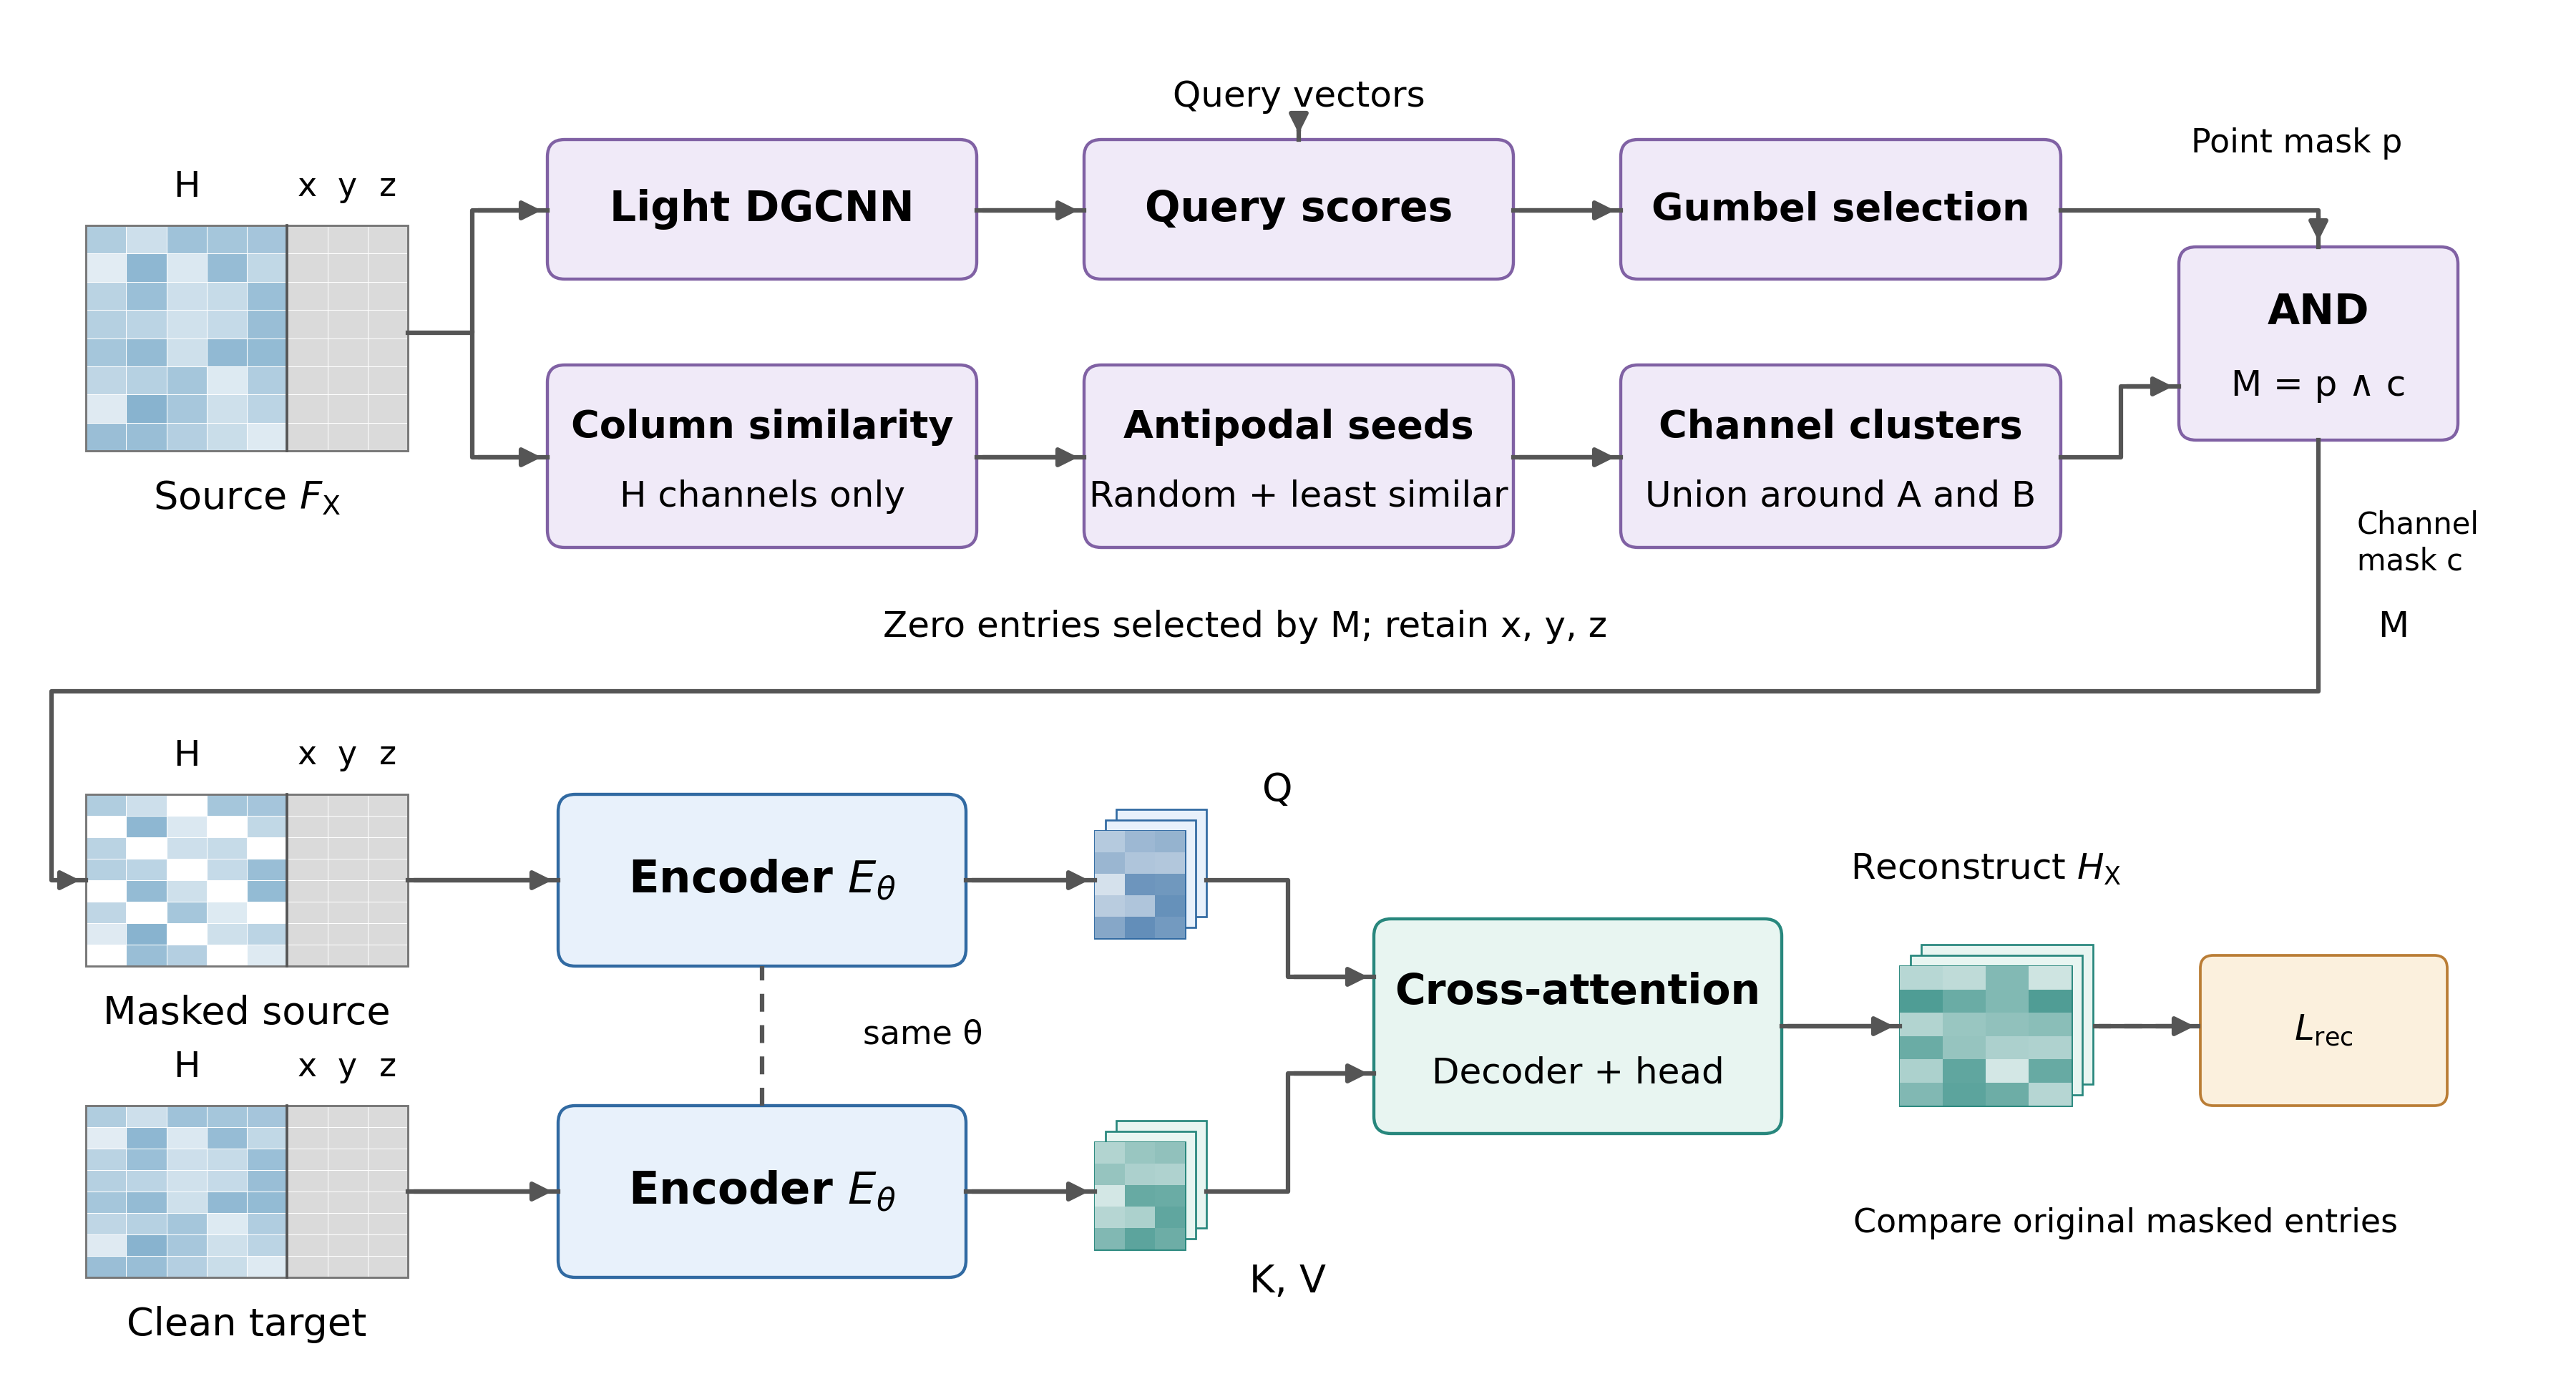
\includegraphics[width=\textwidth]{current/asmae-pipeline.png}
\caption[ASMAE with explicit coordinate conditioning.]{ASMAE and its mask generator. Point selection and descriptor-channel selection jointly define the mask; XYZ remains visible. Masked source tokens query clean target features for reconstruction, also performed in the reverse direction. Both $E_\theta$ blocks denote the same encoder parameters; the mask generator has its own Light DGCNN.}
\label{fig:asmae}
\end{figure}

\subsection{Descriptor masking and cross-reconstruction}
The AAMG mask generator has two selection branches, shown in Figure~\ref{fig:asmae}. A Light DGCNN extracts features for point selection. Query vectors score these features, and hard Gumbel selection chooses point locations. The union of selected locations gives a binary point mask $p_i$.

The second branch computes cosine similarity between descriptor columns, excluding XYZ. It selects a random seed channel and a channel least similar to that seed, then combines channels similar to each seed. This gives a channel mask $c_j$. Their intersection defines the entries to hide:
\begin{equation}
 M_{ij}=p_i\land c_j,\qquad
 \widetilde F_{ij}=\begin{cases}0,&M_{ij}=1,\\ F_{ij},&M_{ij}=0.\end{cases}
\end{equation}
Coordinate channels remain visible, and all point positions are retained. The Light DGCNN belongs to the mask generator; the shared ASMAE encoder $E_\theta$ processes the resulting masked or clean feature matrices.

The masked source representation supplies decoder queries. Clean target embeddings supply keys and values, allowing the decoder to use cross-shape context to reconstruct source descriptors. Exchanging the source and target gives bidirectional reconstruction. This paired masked-learning design is motivated by AMIGO \citep{article}. Separate clean encoder passes supply embeddings for the auxiliary objectives and matching.

\section{Visual Feature Module}
The visual branch projects the point cloud into multiple depth-based views. A frozen DINOv2 backbone extracts patch descriptors \citep{oquab2024dinov2learningrobustvisual}. Visibility testing associates image samples with surface points, and aggregation across views produces a point descriptor $d_i$ with observation confidence $c_i$. Neighbourhood smoothing shares visual context locally.

A prediction head maps each geometric embedding to a visual descriptor $\hat d_i$. Distillation weights the lifted observations by confidence:
\begin{equation}
 L_{\mathrm{DINO}}=
 \frac{\sum_i c_i\,[1-\cos(\hat d_i,d_i)]}{\sum_i c_i}.
\end{equation}
The objective is evaluated on both shapes. At matching time, observation confidence controls the blend of observed and predicted visual features. The visual branch therefore supplies both training supervision and an inference descriptor, following the use of lifted visual information in non-rigid matching \citep{Chen_2025_CVPR}.

\section{Representation Objectives}
\label{sec:objectives}
The representation objectives supervise complementary properties of the shared encoder. Reconstruction uses masked entries, geometric objectives use clean paired embeddings, self-identity uses an augmented observation of the same shape, and visual distillation uses lifted DINOv2 descriptors.

\subsection{Reconstruction and feature separation}
The reconstruction loss measures the absolute error on masked descriptor entries in both directions. A separation term discourages excessive similarity between distinct points. For normalized embeddings $z_i$, its form is
\begin{equation}
 L_{\mathrm{sep}}(Z)=\frac{1}{N(N-1)}\sum_{i\ne j}
 \max(z_i^\top z_j-m,0),
\end{equation}
where $m$ is the similarity margin. Together, these objectives preserve reconstructive information and discrimination between point features.

\subsection{Cycle and intrinsic consistency}
Feature similarities define directional soft maps
\begin{equation}
 P_{XY}=\operatorname{softmax}_{j}(Z_XZ_Y^\top/\tau),
\end{equation}
with temperature $\tau$. The reverse map is constructed analogously. The cycle objective measures coordinate recovery after mapping in both directions:
\begin{equation}
 L_{\mathrm{cycle}}=\operatorname{MSE}(P_{XY}P_{YX}X,X)
 +\operatorname{MSE}(P_{YX}P_{XY}Y,Y).
\end{equation}

For intrinsic consistency, the soft map transports the target biharmonic embedding to source indexing, $\widetilde\Psi_X=P_{XY}\Psi_Y$. The directional distortion is
\begin{equation}
 L_B(X,Y)=\underset{i,j}{\operatorname{mean}}
 \left|d_B^X(i,j)-\|\widetilde\psi_X(i)-\widetilde\psi_X(j)\|_2\right|.
\end{equation}
Averaging the two directions encourages matched points to preserve the intrinsic relationships within each shape.

\subsection{Local orientation consistency}
Neighbouring source points form triplets with directed area vectors. Their soft-mapped triplets define corresponding vectors in the aligned target frame. An angular agreement term compares the normalized vectors. This supplies a local directional constraint alongside the distance-based objective.

\subsection{Self-identity supervision}
The self-identity branch uses the same ASMAE encoder $E_\theta$ as reconstruction and clean feature extraction. It reuses the clean source embedding $Z_X=E_\theta(F_X,X)$ and computes an additional embedding for an augmented source subset. Both passes share parameters and receive gradients from the identity objective.

A clean shape and an augmented subset share point identities. Rotation, scaling and coordinate perturbations change the observation while retaining the correspondence of sampled vertices. An InfoNCE objective \citep{Oord_2018_CPC} treats the matching point as a positive candidate:
\begin{equation}
 L_{\mathrm{self}}=-\frac{1}{|Q|}\sum_{i\in Q}
 \log\frac{\exp(z_i^\top z'_{\pi(i)}/\tau_s)}
 {\sum_j\exp(z_i^\top z'_j/\tau_s)}.
\end{equation}
Here $Q$ contains queried source identities retained in the subset, $\pi(i)$ is the subset position of the same original vertex, and $\tau_s$ controls the contrastive distribution. Embeddings are normalized before comparison. Cross-entropy rewards the matching identity against all other points in the augmented subset. The objective is evaluated on the source member of each ordered training pair.

\subsection{Joint optimization}
Representation learning combines the objectives through weights $\lambda_j$:
\begin{equation}
 L_{\mathrm{rep}}=\sum_{j\in\mathcal J}\lambda_jL_j,
 \quad\mathcal J=\{\mathrm{rec,sep,cycle},B,\mathrm{orient,self,DINO}\}.
\end{equation}
Training first establishes relative orientation and then introduces the representation objectives progressively. The overall objective combines $L_{\mathrm{rep}}$ with OEM and domain supervision. This separates the supervision of alignment from the learning of point descriptors while connecting both through the aligned inputs.

\section{Heat-Anchored Deformation Matching}
\label{sec:hadm}
HADM converts geometric and visual embeddings into a dense point map through orientation selection, anchor propagation and deformation refinement.

\subsection{Orientation selection and feature fusion}
Predictions from independently sampled point subsets contribute orientation votes. Candidate alignments include strong angular modes and a half-turn alternative. For each candidate, the target is aligned and encoded. Intrinsic anchor agreement and feature similarity jointly score the candidate, and the selected alignment supplies the pair for refinement.

Observed and predicted visual descriptors are blended using their confidence. A shared dimensionality reduction places the visual features of both shapes in a common compact representation. Normalized geometric and visual feature blocks are then fused for correspondence search.

\subsection{Intrinsic anchor consistency}
Mutual feature matches propose anchor pairs. Similarity margins rank their confidence, while spatial coverage in biharmonic space distributes candidates across the shape. Agreement between candidate pairs is measured by
\begin{equation}
 W_{uv}=\exp\left[-\frac{
 (d_B^X(a_u,a_v)-d_B^Y(b_u,b_v))^2}{2\sigma_c^2}\right].
\end{equation}
A spectral score identifies mutually compatible candidates, and consistency filtering forms the anchor set. This uses the pairwise-compatibility principle of spectral matching \citep{Leordeanu_2005_Spectral}.

\subsection{Anchor propagation}
Corresponding anchors define proximity descriptors on both shapes:
\begin{equation}
 h_{j,\sigma}(x)=\exp\left[-\frac{
 \|\psi(x)-\psi(a_j)\|_2^2}{2\sigma^2}\right].
\end{equation}
These Gaussian responses encode position relative to the anchor set in biharmonic space. Combining them with point features transfers anchor information to other locations. Successive stages expand and refine the anchor set using this additional context.

\subsection{Deformation and dense assignment}
A similarity transformation estimated from the anchors initializes source alignment. A deformation graph then represents non-rigid adjustment through local node transformations \citep{10.1145/1275808.1276478}. Each point blends nearby transformations to obtain its deformed position. Positional agreement and anchor constraints guide the fit, while as-rigid-as-possible regularization encourages compatible motion between neighbouring graph nodes \citep{sorkine2007rigid}. Refinement proceeds from a coarse graph to finer spatial detail.

The final map combines fused feature similarity with deformed positional agreement:
\begin{equation}
 T(i)=\arg\max_j\left[G_X(i)^\top G_Y(j)
 -\lambda_p\|\widetilde x_i-y_j\|_2^2\right].
\end{equation}
Here $G$ contains the fused features and anchor-relative descriptors, and $\widetilde X$ is the deformed source. The resulting point indices support attribute transfer between shapes, as illustrated by the colour-transfer operation in Figure~\ref{fig:current-pipeline}.
